\documentclass[a4paper,12pt]{article} % тип документа

%  Русский язык
\usepackage[T2A]{fontenc}			% кодировка
\usepackage[utf8]{inputenc}			% кодировка исходного текста
\usepackage[english,russian]{babel}	% локализация и переносы

\usepackage{graphicx, scalerel}               % импорт изображений
\usepackage{wrapfig}                % обтекаемые изображения
\graphicspath{{pictures/}}          % обращение к подкаталогу с изображениями
\usepackage[14pt]{extsizes}         % для того чтобы задать нестандартный 14-ый размер шрифта
\usepackage[warn]{mathtext}         % русский язык в формулах
\usepackage{indentfirst}            % indent first
\usepackage[margin = 25mm]{geometry}% отступы полей
\usepackage[table,xcdraw]{xcolor}   % таблицы
\usepackage{amsmath,amsfonts,amssymb,amsthm,mathtools} % Математика
\usepackage{wasysym}                % ???
\usepackage{upgreek}                % ???  
\usepackage{caption}
\usepackage{multirow}
\captionsetup{labelsep=period}
\usepackage[font=small,labelfont=bf]{caption}
\usepackage{gensymb} % degree symbol
\usepackage{tikz}
\usetikzlibrary{positioning}


\begin{document}
	
	
	\begin{center}
		
		\textbf{НАЦИОНАЛЬНЫЙ ИССЛЕДОВАТЕЛЬСКИЙ УНИВЕРСИТЕТ \\ <<МОСКОВСКИЙ ФИЗИКО-ТЕХНИЧЕСКИЙ ИНСТИТУТ>>}
		\vspace{13ex}
		
		\textbf{Лабораторная работа 5.5.5\\ <<$\gamma$-спектроскопия>>}
		\vspace{40ex}
		
		\normalsize{Шумаков Иван Игоревич \\ студент группы Б01-009\\ 3 курс ФРКТ\\}
	\end{center}
	
	\vfill 
	
	\begin{center}
		г. Долгопрудный\\ 
		2022 г.
	\end{center}
	
	
	\thispagestyle{empty} % выключаем отображение номера для этой страницы
	\newpage

	\textbf{Цель работы:} Исследовать электронный парамагнитный резонанс в молекуле дифенилпикрилгидразила $C_{18}H_{12}N_50_6$, определить $g$-фактор электрона. 

  \section{Теоретические сведения}
    В квантовой теории проекция момента импульса M на заданную ось (обычно ее принимают за ось z) может принимать лишь дискретные значения
    \begin{equation}
      M_z = m \hbar \quad
      m = 0, \pm 1, ... , \pm l
    \end{equation}
    Посколку операторы проекций момента импульса на оси не коммутирут, они не могут быть одновременно точно определены.
    Таким образом одновременно только проекция на одну ось и длинна вектора момента импульса могут быть точно определены.\par
    Квадрат момента импульса (а следовательно, и его модуль) квантуется в соответствии с формулой
    \begin{equation}
      M^2 = \hbar^2 l(l + 1)
    \end{equation}
    Число l, определяющее возможные значения квадрата момента и равное максимальному значению числа m, называется орбитальным квантовым числом.\par
    В магнитном поле H0 магнитный диполь µm обладает потенциальной энергией
    \begin{equation}
      E = - (\mu_m, H_0)
    \end{equation}
    Следовательно, для «магнитной» частицы, характеризуемой квантовым числом J, в магнитном поле возникает 2J + 1 энергетических уровней — зеемановских уровней.
    \begin{figure}[h!]
      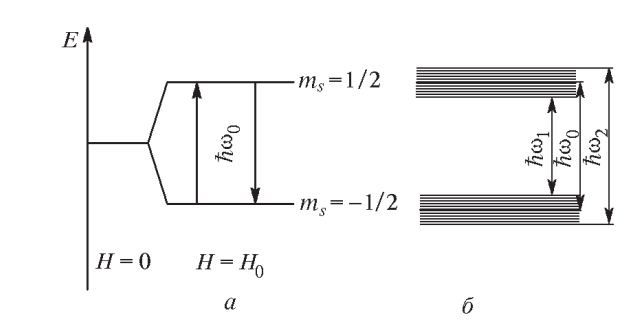
\includegraphics[width=0.7\textwidth]{img/Levels.png}
      \centering
      \caption{Схема расщепления уровней}
    \end{figure}\par
  \newpage 
    Простейшей моделью рассмотрения ЭПР является система из невзаимодействующих частиц со спином $S = 1/2$, помещенная во внешнее магнитное поле. 
    В отсутствии поля проекции спинов на ось совпадают, как и энергии. 
    При подаче магнитного поля и эффекта Зеемана энергии с различными направлениями спина начинают различаться. 
    А если мы в систему направим поток фотонов с этой энергией разности этих энергий, то станут возможны индуцированные переходы межу этими состояниями. 
    Для наблюдения этого поглощения необходимо резонансное совпадение частоты излучения с зеемановским расщеплением спиновых подуровней.
    Измеряемой в эксперименте величиной является поглощаемая в образце мощность излучения. 
    Для увеличения точности измерения желательно увеличить эту поглощаемую мощность.
    Поглощение переменного магнитного поля в образце описывается мнимой частью магнитной восприимчивости
    \begin{equation}
      P_{\text{погл}} = \frac{1}{2}\omega b^2 \chi''(\omega, B)
    \end{equation}
    где $\omega$ --- частота переменного поля, $b$ --- амплитуда однородного по малому образцу переменного поля, $B$ --- постоянное магнитное поле, $\chi''$ ---  мнимая часть высокочастотной магнитной восприимчивости. 
    Магнитная восприимчивость связывает намагниченность $\vec{m}$ с подмагничивающим магнитным полем $\vec{b} : \vec{m} =\chi \vec{b}$. 
    Комплексное представление восприимчивости имеет смысл для описания отклика на переменное поле $\vec{b}=\vec{b}_0 \cdot e^{-i \omega t}$. 
    Тогда $\vec{m} =\chi \vec{b} = (\chi' + i \chi'')\vec{b}_0 e^{-i \omega t}=\chi' \vec{b}_0 e^{-i \omega t} + \chi'' \vec{b}_0 e^{-i \omega t + \frac{pi}{2}}$. 
    Таким образом, действительная часть высокочастотной восприимчивости описывает вклад в намагниченность, находящийся в фазе с подмагничивающим полем, а мнимая часть — вклад, сдвинутый относительно подмагничивающего поля по фазе на $\frac{\pi}{2}$. 
    Естественно, при $\omega=0$ мнимая часть восприимчивости $\chi'' = 0$. 
    Сдвиг по фазе отклика (намагниченности) относительно вынуждающей силы (переменного поля) связан с потерями энергии, поэтому мнимая часть восприимчивости является мерой диссипации энергии в системе.
    Простейшей системой для изучения методом ЭПР является парамагнетик — система слабо взаимодействующих атомов, ионов или молекул, обладающих собственным магнитным моментом. 
    Пренебрегая взаимодействием, можно рассмотреть поведение магнитного диполя в постоянном и переменном магнитном поле. 
    В «классическом» подходе рассматривается прецессия магнитного момента во внешнем поле
    при отклонении магнитного момента от равновесия. Классический магнитный диполь
    стремится выровняться вдоль силовых линий магнитного поля, при отклонении от
    равновесия возникает возвращающий механический момент $\vec{T}=\vec{M}\times \vec{B}$ . Так как
    магнитный и механический момент иона связаны друг с другом гиромагнитным отношением
    $\gamma$ как $\vec{M} =\gamma \vec{I}$ , где $\vec{I}$ - это полный момент импульса, то с учётом уравнения динамики $\frac{d\vec{I}}{dt} = \vec{T}$ получим уравнение прецессии магнитного момента $\frac{d\vec{M}}{dt} = \gamma \vec{M}\times \vec{B}$. Аналогично
    с известной задачей о прецессии гироскопа можно заметить, что при отклонении магнитного
    момента от направления магнитного поля возникает незатухающая прецессия вокруг
    направления поля с угловой скоростью $\vec{\Omega}= - \gamma \vec{B}$ , частота этой прецессии $\Omega_L=\gamma B$
    называется ларморовской. При совпадении частоты переменного поля с ларморовской
    частотой возможно возникновение резонансного поглощения.
    Расщепление терма свободного иона (или молекулы) определяется спектроскопическим
    фактором Ланде ($g$-фактором Ланде): $E(m_J)=g\mu_B B m_J$.
    \begin{equation}
      g_{\text{эфф}} = \frac{h \nu}{\mu_B B}
    \end{equation}
  
    \section{Экспериментальная установка}
    
    Образец (порошок ДФПГ) в стеклянной ампуле помещяется внутрь катушкииндуктивнсоти входящей в состав колебательного контура. 
    Входящий в состав контура конденсатор состоит из двух платсин, разделенных воздушным зазором, одна из пластин может перемещаться поворотом штока. 
    Колебания в контуре возбуждаются антенной, соединённой с генератором частоты (ВЧ) Г4-116. 
    Амплитуда колебаний поля в катушке индуктивности измеряется по наводимой в петле связи ЭДС индукции. 
    Высокочастотные колебания ЭДС индукции в приёмном контуре детектируются диодом, измеряемая при помощи осциллографа низкочастотная огибающая этого сигнала пропорциональна квадрату амплитуды колебаний поля в катушке.
    \begin{figure}[h!]
      \centering
      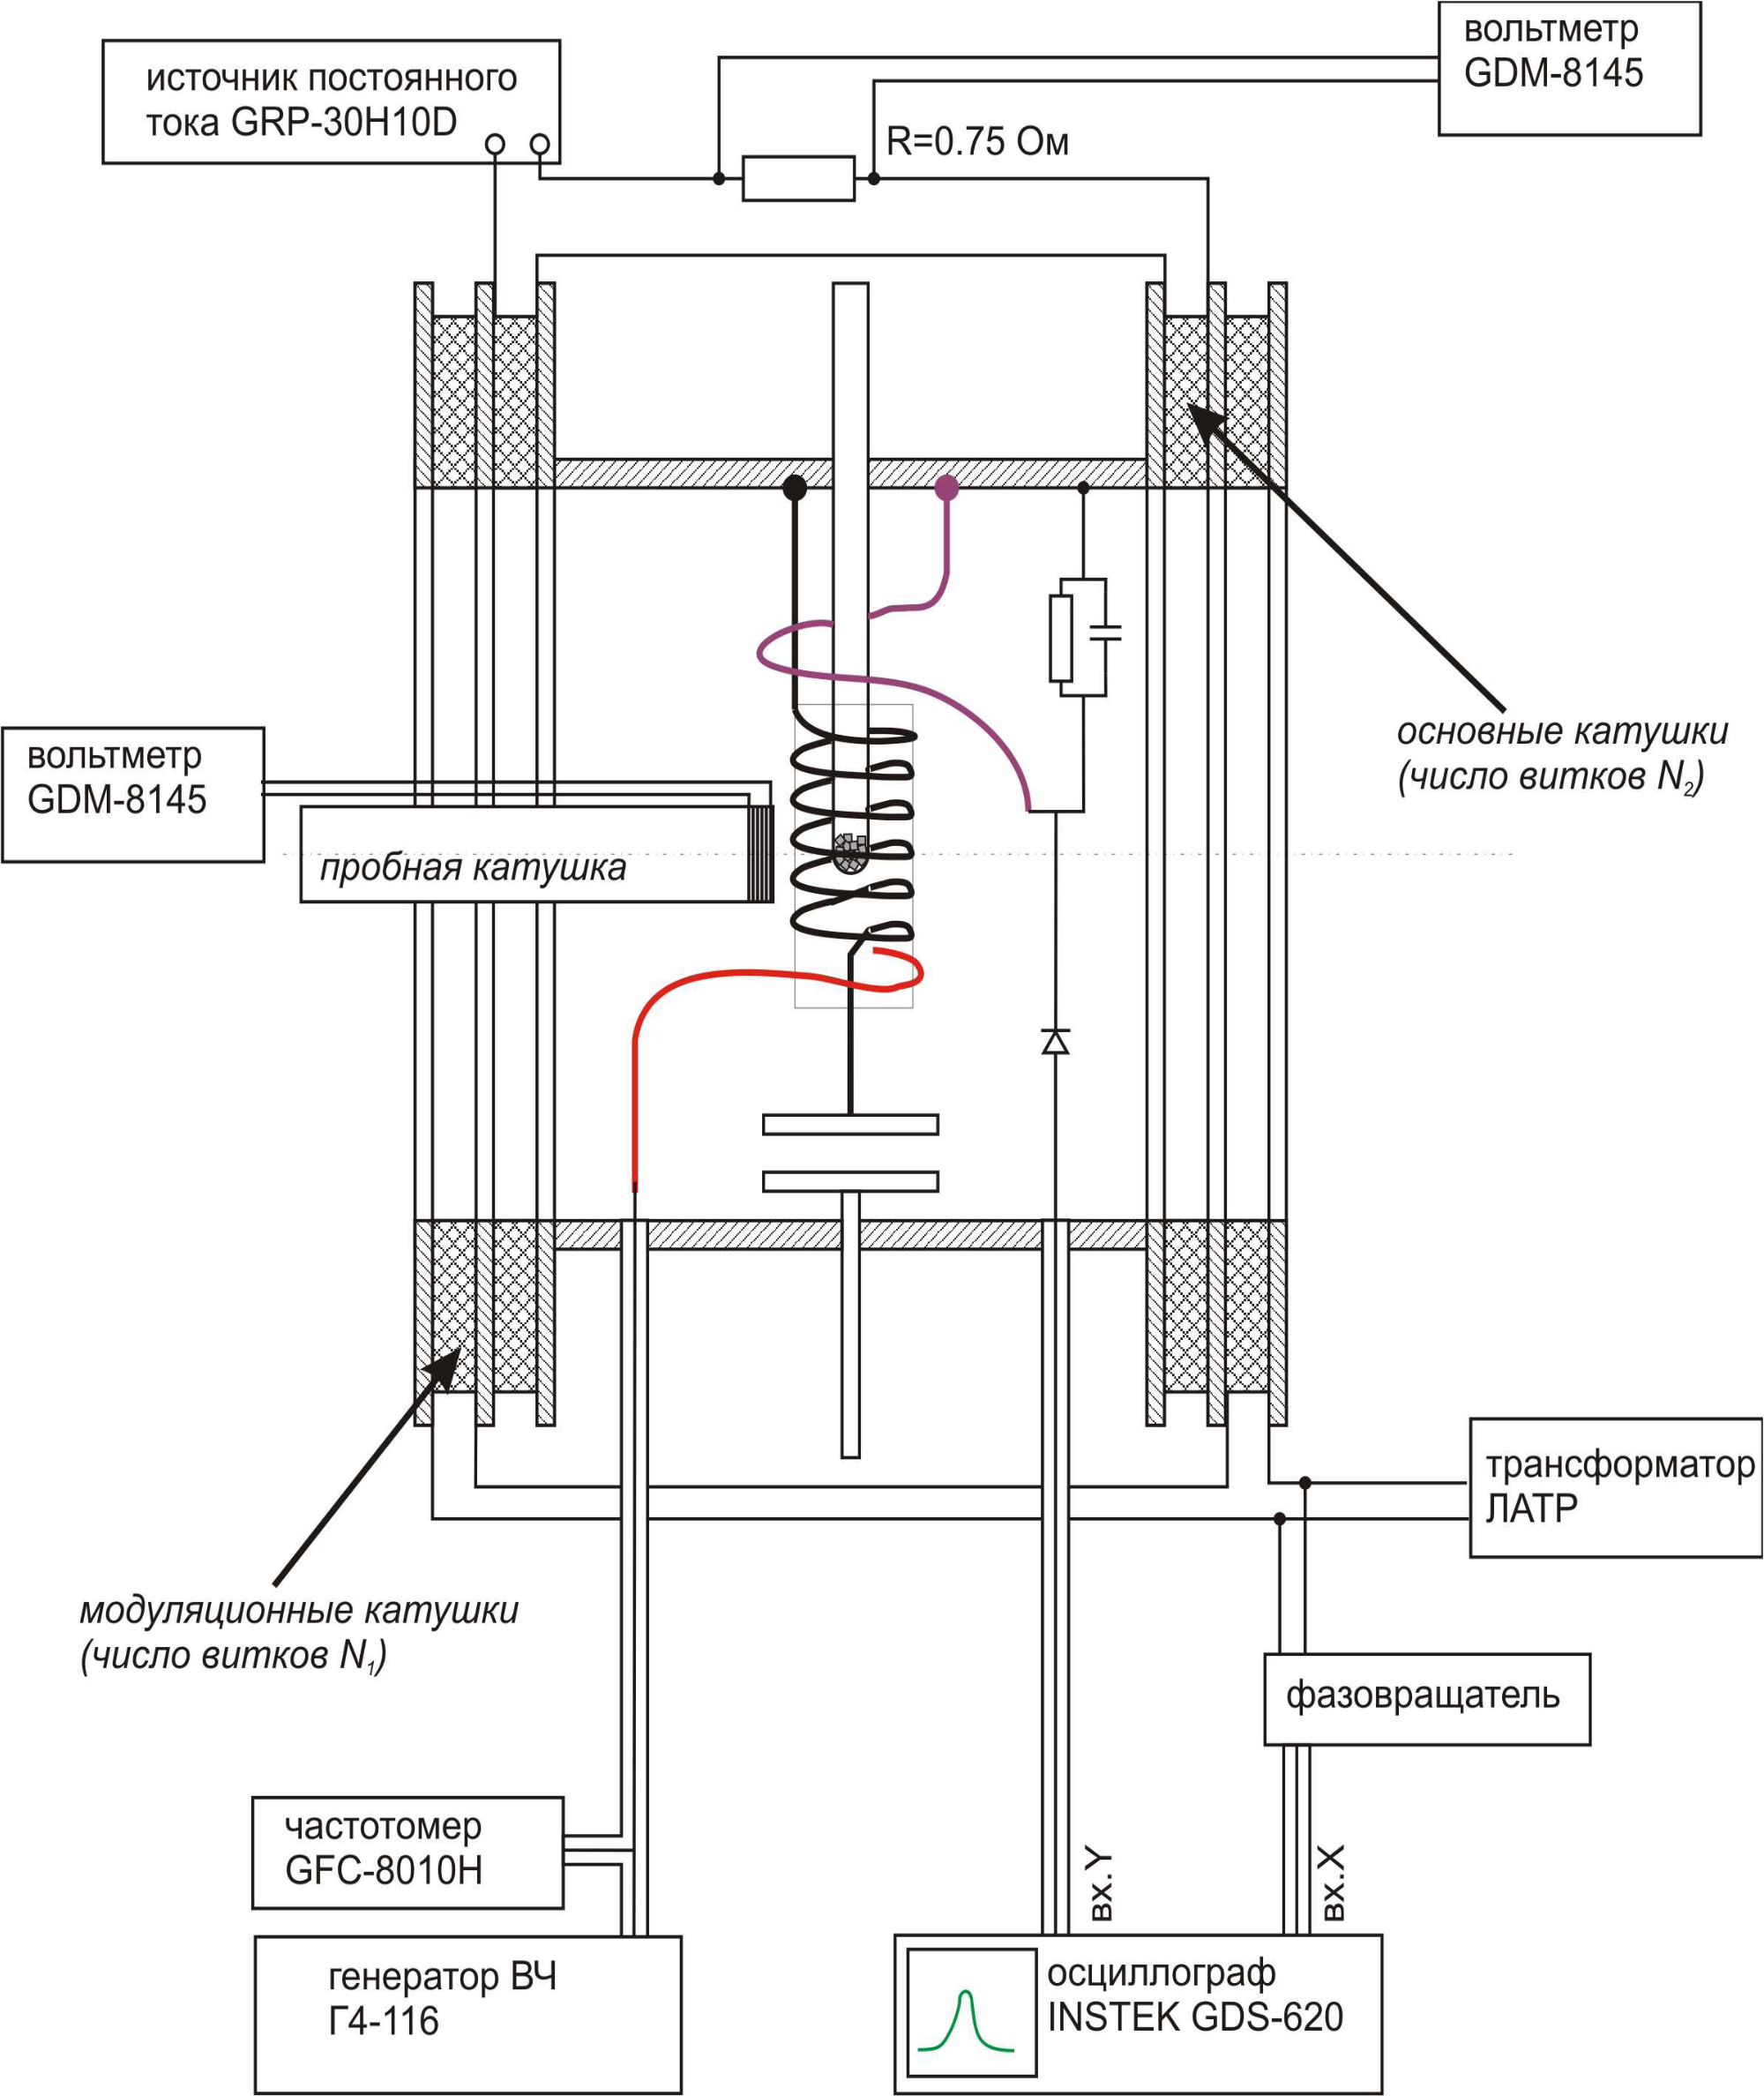
\includegraphics[scale=0.17]{img/equip.png}
      \caption{Схема установки}
    \end{figure}
    Постоянной магнитное поле создаётся пропусканием тока от источника постоянного тока через основные катушки. 
    При этом при помощи вольтметра измеряется падение напряжения на резисторе в цепи основных катушек. 
    Переменное поле небольшой амплитуды создаётся подачей на модуляционные катушки напряжения с регулируемого трансформатора ЛАТР. 
    Для измерения амплитуды колебаний переменного поля используется пробная катушка известной геометрии, подключенная к вольтметру.\par
    \begin{table}[h!]
      \centering
      \begin{tabular}{|l|l|l|}
      \hline
      \textbf{Катушка} & $N$ & $D$, см \\ \hline \hline
      Основная         & 6700         & $25\pm1$             \\ \hline
      Модуляционная    & 5000         & $30\pm1$             \\ \hline
      Пробная          & 45           & $1.52\pm0.01$             \\ \hline
      \end{tabular}
      \caption{Параметры катушек.}
    \end{table}

  \section{Ход работы}
    В данной работе измерялось поглощение э-м поля на резонансной частоте.
    Первоначально генератор был настроен на частоту колебательного контура:
    \begin{equation}
      f_0 = (164 \pm 1) МГц
    \end{equation}
    Подберем величину постоянного магнитного поля в катушках так, чтобы наблюдался сигнал резонанского поглощения. 
    Для этого подадим на катушки достаточное напряжение.
    При резонансе напряжение на резисторе в цепи основных катушек:
    \begin{equation}
      U_0 = (130 \pm 1) \ \text{мВ}.
    \end{equation}\par
    По осциллографу была определена ширина линии ЭПР. 
    Погрешность ширины линии в основном обусловлена погрешностью измерений амплитуд по экрану осциллографа: 
    \begin{equation}
      \begin{gathered}
          A_\text{полн} = 10 \pm 0.2 \ \text{дел}, \ A_{1/2} = 3 \pm 0.2 \ \text{дел} \\
          B_\text{мод} = \sqrt{2} \frac{2\varepsilon}{\pi^2d^2N\nu} = 0.75\pm 0.05 \text{мТл},
      \end{gathered}
    \end{equation}
    \begin{equation}
      \Delta B = \frac{A_{1/2}}{A_{\text{полн}}}B_\text{мод} = 0.22 \pm 0.02 \ \text{мТл},
    \end{equation}
    где $A_\text{полн}$ -- полный размах модулирующего поля, $A_{1/2}$ -- ширина кривой на полувысоте, $B_\text{мод}$ -- амплитуда модулирующего поля,
    $\varepsilon$ -- ЭДС индукции при внесении пробной катушки, $N$ -- число витков катушки, $d$ -- диаметр катушки, $\nu$ -- частота модулирующего напряжения (50 Гц).\par
    Для определения связи падения напряжения на резисторе в цепи основных катушек и магнитным полем в центре магнита была использована пробная катушка.
    По полученным данным была построен график зависимости напряжения на катушке(V) от напряжения на сопротивлении ($V_R$):
    \begin{table}[h!]
      \centering
      \begin{tabular}{|c|c|c|}
      \hline
      \textbackslash{} & $V_R$ мВ & $V$ мВ \\ \hline
      1                & 3.52     & 0.44   \\ \hline
      2                & 5.35     & 0.65   \\ \hline
      3                & 7.14     & 0.85   \\ \hline
      4                & 8.90     & 1.07   \\ \hline
      5                & 10.53    & 1.25   \\ \hline
      \end{tabular}
    \end{table}
    \begin{figure}[h!]
      \centering
      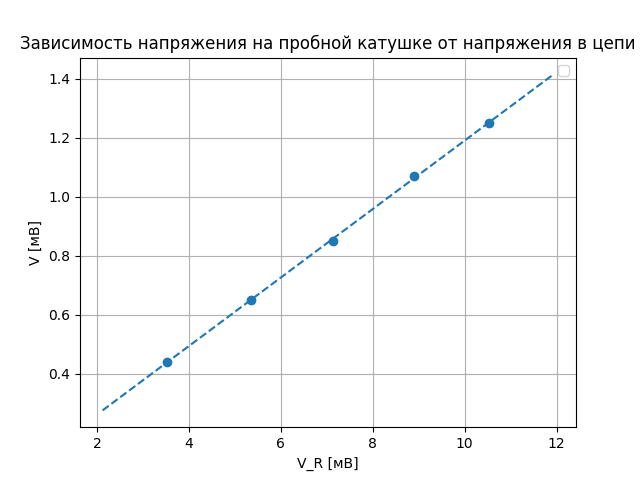
\includegraphics[scale=0.65]{img/Gra.png}
      \caption{Калибровочный график}
    \end{figure}
    Значение коэффициента наклона 
    \[ k = (11.7 \pm 0.1) \cdot 10^{-2} \]
    Рассчитав поле, создаваемое основными катушками,
    \begin{equation*}
        B_0 = \frac{4 k U_0}{2\pi\nu N \pi d^2} = (6.1 \pm 0.1) \text{мТл}.
    \end{equation*}
    Найдем $g$-фактор электрона:
    \begin{equation*}
        g = \frac{hf_0}{\mu_BB_0} = 1.9 \pm 0.1
    \end{equation*}

  \section*{Вывод}
    В данной работе был исследован ЭПР в молекуле ДФПГ, определяется $g$-фактор электрона $\pmb{g = 1.9 \pm 0.1}$, а также измерена ширина линий ЭПР $\Delta B = 0.22 \pm 0.2~\text{мТл}$. 
	  Измеренный $g$-фактор электрона совпадает с табличным значением для свободного электрона: $\pmb{g_{free} = 2,0}$. 
    Это обусловлено тем, что ПР происходит на неспаренных электронах так же, как на свободных.

\end{document}